\documentclass{article}
\usepackage[utf8]{inputenc}
\usepackage{graphicx}
\usepackage{amsmath}
\usepackage{amssymb}
\usepackage{amsthm}

\title{Computational Physics (physics760)\\Exercise 3}
\author{Ajay S. Sakthivasan, Dongjin Suh}
\date{November 18, 2022}

\begin{document}

\maketitle

\section{Applying HMC to the long-range Ising model}

\begin{enumerate}
\item Derive expressions for O$[\phi]$ for mean magnetization (per site) and energy (per site)

\begin{flalign*}
Z[J > 0] &= \int_{-\infty}^{\infty} \frac{d\phi}{\sqrt{2\pi \beta J}} \mathrm{e}^{-\frac{\phi^2}{2\beta J} +N\log(2\cosh{(\beta h \pm \phi)})} &\\
&\\
\langle O\rangle &= \frac{1}{\mathrm{Z}} \int_{}^{} \frac{d\phi}{\sqrt{2\pi \beta J}} O[\phi] \mathrm{e}^{-S[\phi]}&\\
&\\
&\textbf{Mean Magnetization:} &\\
\langle m\rangle &= \frac{1}{N\beta} \frac{\partial}{\partial h} \log (\mathrm{Z}) &\\
\langle m\rangle &= \frac{1}{N\beta} \frac{\partial}{\partial h} \log\left( \int_{-\infty}^{\infty} \frac{d\phi}{\sqrt{2\pi \beta J}} \mathrm{e}^{-\frac{\phi^2}{2\beta J} +N\log(2\cosh{(\beta h \pm \phi)})}\right) &\\
&= \frac{1}{N\beta} \frac{1}{\mathrm{Z}} \int_{-\infty}^{\infty} \frac{d\phi}{\sqrt{2\pi \beta J}} \frac{\partial}{\partial h} \mathrm{e}^{-\frac{\phi^2}{2\beta J} +N\log(2\cosh{(\beta h \pm \phi)})}&\\
&= \frac{1}{N\beta} \frac{1}{\mathrm{Z}} \int_{-\infty}^{\infty} \frac{d\phi}{\sqrt{2\pi \beta J}} \mathrm{e}^{-\frac{\phi^2}{2\beta J} +N\log(2\cosh{(\beta h \pm \phi)})}\\
&\qquad\frac{\partial}{\partial h} \left(-\frac{\phi^2}{2\beta J} +N\log(2\cosh{(\beta h \pm \phi)})\right)&\\
&= \frac{1}{\mathrm{Z}} \int_{-\infty}^{\infty} \frac{d\phi}{\sqrt{2\pi \beta J}} \mathrm{e}^{-\frac{\phi^2}{2\beta J} +N\log(2\cosh{(\beta h \pm \phi)})} \frac{1}{N\beta} N\beta \tanh{(\beta h \pm \phi)} &\\
&= \frac{1}{\mathrm{Z}} \int_{}^{} \frac{d\phi}{\sqrt{2\pi \beta J}} O[\phi] \mathrm{e}^{-S[\phi]} = \langle O\rangle &\\
\implies O[\phi] &= \tanh{(\beta h \pm \phi)}&
\end{flalign*}
\begin{flalign*}
&\textbf{Average Energy:} &\\
\langle \epsilon \rangle &= -\frac{1}{N} \frac{\partial}{\partial \beta} \log (\mathrm{Z})&\\
\langle \epsilon \rangle &= -\frac{1}{N} \frac{\partial}{\partial \beta} \log\left( \int_{-\infty}^{\infty} \frac{d\phi}{\sqrt{2\pi \beta J}} \mathrm{e}^{-\frac{\phi^2}{2\beta J} +N\log(2\cosh{(\beta h \pm \phi)})}\right) &\\
&= -\frac{1}{N} \frac{1}{\mathrm{Z}} \int_{-\infty}^{\infty} d\phi \frac{\partial}{\partial \beta} \frac{1}{\sqrt{2\pi \beta J}} \mathrm{e}^{-\frac{\phi^2}{2\beta J} +N\log(2\cosh{(\beta h \pm \phi)})} &\\
&= \frac{1}{\mathrm{Z}} \int_{-\infty}^{\infty} \frac{d\phi}{\sqrt{2\pi \beta J}} \mathrm{e}^{-\frac{\phi^2}{2\beta J} +N\log(2\cosh{(\beta h \pm \phi)})} \left(-\frac{2NhJ\beta^2\tanh{(\beta h \pm \phi)} - J\beta + \phi^2}{2NJ\beta^2} \right)&\\
&= \frac{1}{\mathrm{Z}} \int_{}^{} \frac{d\phi}{\sqrt{2\pi \beta J}} O[\phi] \mathrm{e}^{-S[\phi]} = \langle O\rangle &\\
\implies O[\phi] &= -\frac{2NhJ\beta^2\tanh{(\beta h \pm \phi)} - J\beta + \phi^2}{2NJ\beta^2} &
\end{flalign*}

\item{Equations of Motion determined using Hamilton's equations}

\begin{flalign*}
&\text{We have,}&\\
\mathcal{H} &= \frac{p^2}{2} + \frac{\phi^2}{2\beta\hat{J}} - N\log(2\cosh{\beta h + \phi})&\\
&\text{Using Hamilton's equation,}&\\
(1)\quad\dot{\phi} &= \frac{\partial}{\partial p} \mathcal{H}&\\
&= \frac{\partial}{\partial p} \left(\frac{p^2}{2} + \frac{\phi^2}{2\beta\hat{J}} - N\log(2\cosh{\beta h + \phi})\right)&\\
\implies \dot{\phi} &= p&\\
(2)\quad\dot{p} &= -\frac{\partial}{\partial \phi} \mathcal{H}&\\
&= -\frac{\partial}{\partial \phi} \left(\frac{p^2}{2} + \frac{\phi^2}{2\beta\hat{J}} - N\log(2\cosh{\beta h + \phi})\right)&\\
&= -\frac{\phi}{\beta\hat{J}} + \frac{N}{2\cosh{(\beta h + \phi)}} 2\sinh{(\beta h + \phi)}&\\
\implies \dot{p} &= -\frac{\phi}{\beta\hat{J}} + N\tanh{(\beta h + \phi)}&
\end{flalign*}

\item{Implementation of Leapfrog algorithm}

The leapfrog algorithm was implemented and the following plot, \ref{fig:lf_conv}, was obtained to verify the given convergence rate of the algorithm.
\begin{figure}[h!]
    \centering
    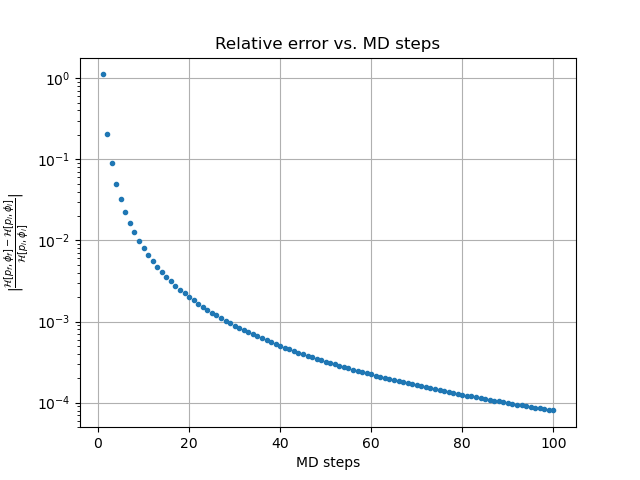
\includegraphics[width = .8\linewidth]{leapfrog_conv.png}
    \caption{Relative error in the energy vs. MD steps}
    \label{fig:lf_conv}
\end{figure}

\newpage

\item{Calculation of the average energy and mean magnetization per site}

With the implemented leapfrog integrator, we coded up the HMC algorithm for the long-range Ising model. \\
We calculated the average energy per site and mean magnetization per site as a function of the coupling factor J=($\beta$J) from 0.2 to 2 by using the HMC algorithm. We set the internal field h = ($\beta$h) as 0.5 and $\beta$ is set as 1 as it can be seen. Also we are using some values of number of sites N ranging from 5 to 20. \\ 
In the following plots are shown the mean magnetization and average energy per site once against J and then against $J^{-1}$ and also the analytical results. 
We used the bootstrap method to calculate the corresponding errors.

\begin{figure}[htbp]
    \centering
    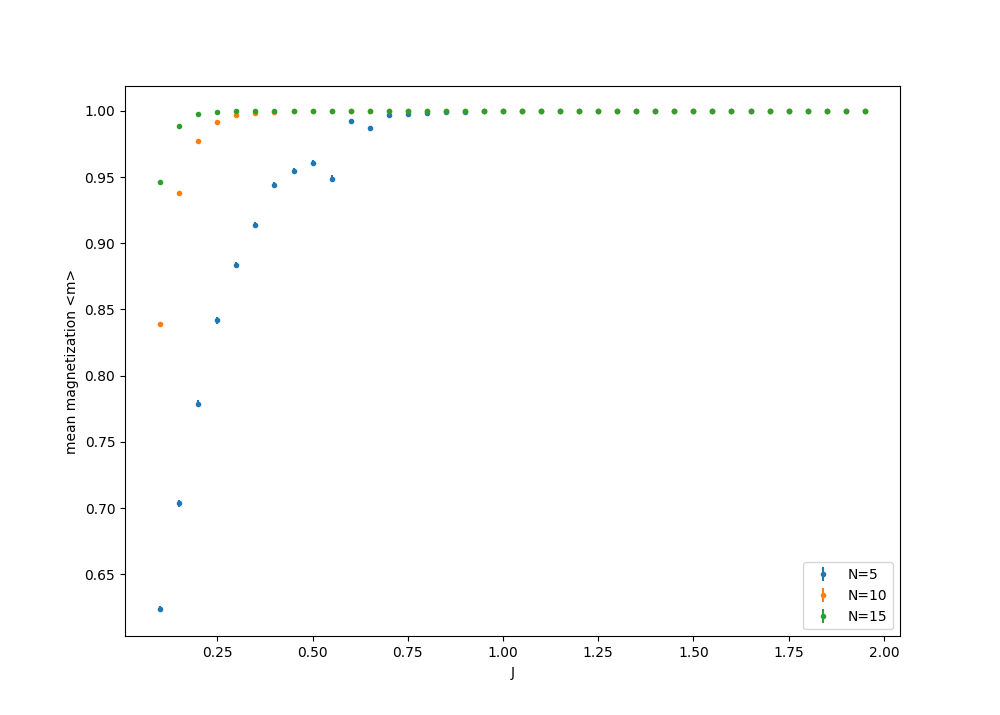
\includegraphics[width = .8\linewidth]{mag_vs_J.png}
    \caption{simulation of mean magnetization vs. J for different N values}
    \label{fig:mag_J}
\end{figure}
\begin{figure}[htbp]
    \centering
    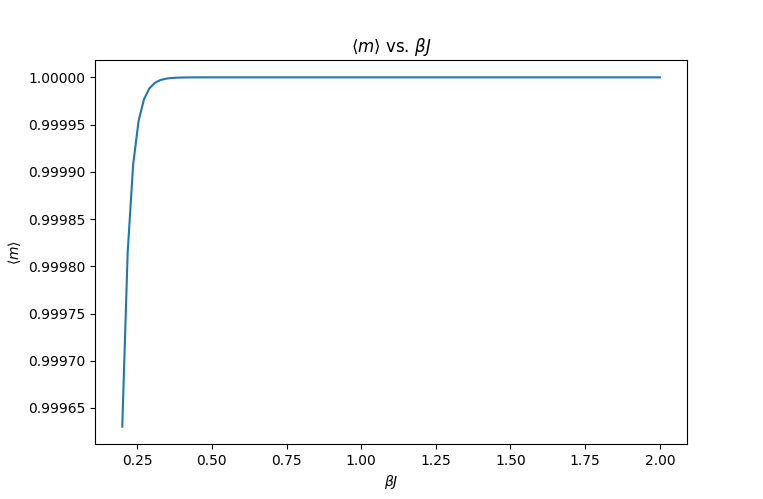
\includegraphics[width = .8\linewidth]{analytic_mag.png}
    \caption{analytical result of average energy vs. J}
    \label{fig:anal_mag}
\end{figure}

\begin{figure}[htbp]
    \centering
    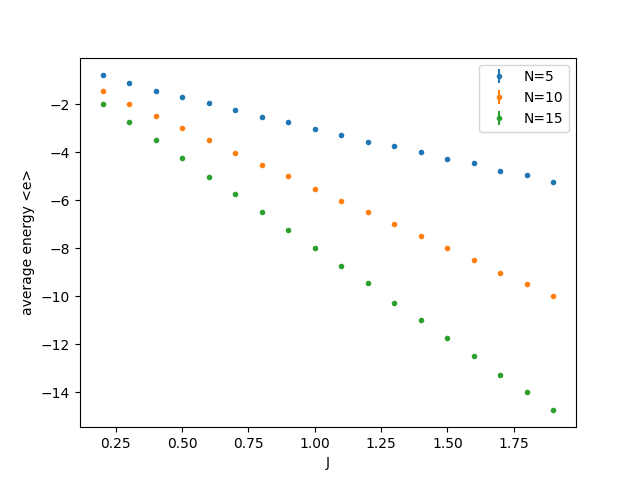
\includegraphics[width = .8\linewidth]{energy_J.png}
    \caption{simulation of average energy vs. J}
    \label{fig:ener_J}
\end{figure}
\begin{figure}[htbp]
    \centering
    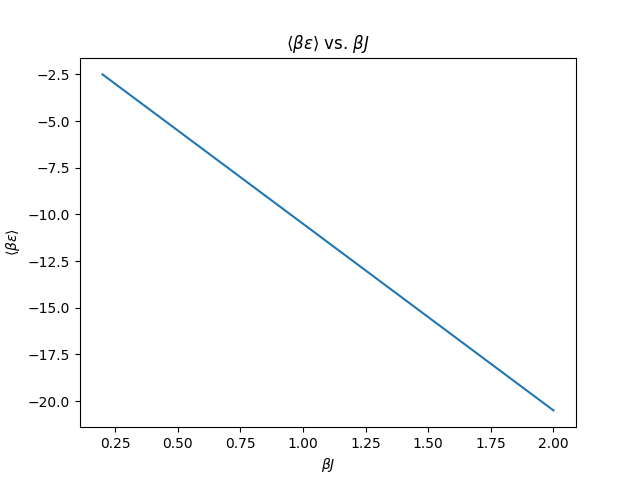
\includegraphics[width = .8\linewidth]{analytic_energy.png}
    \caption{analytical result average energy vs. $J^{-1}$}
    \label{fig:anal_ener}
\end{figure}

\begin{figure}[htbp]
    \centering
    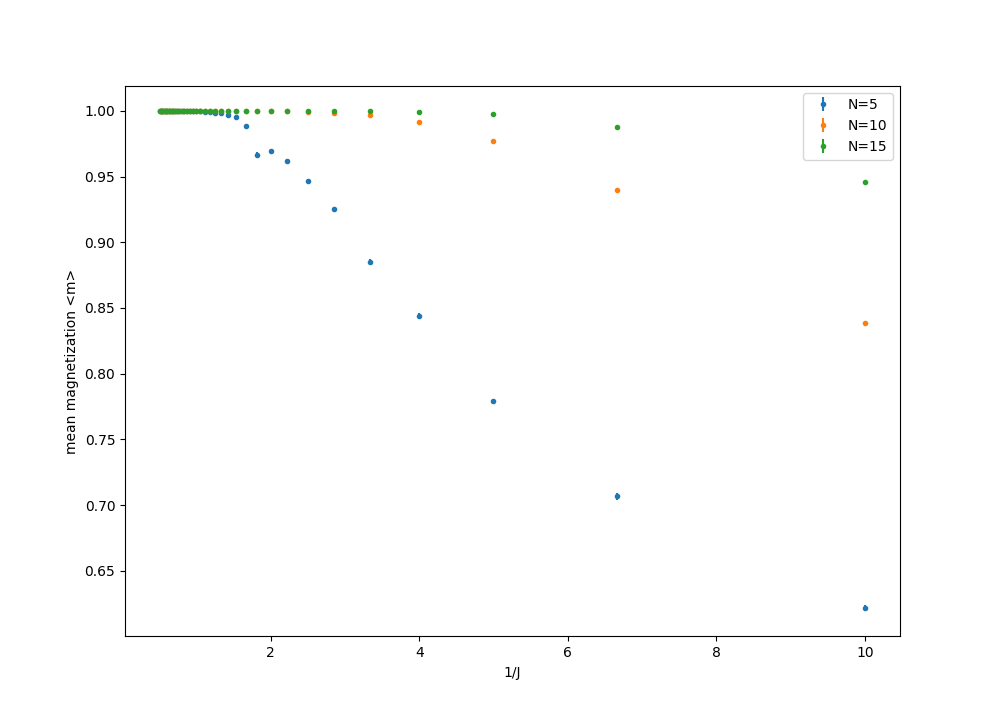
\includegraphics[width = .8\linewidth]{mag_vs_J^-1.png}
    \caption{mean magnetization vs. $J^{-1}$}
    \label{fig:mag_J-1}
\end{figure}
\begin{figure}[htbp]
    \centering
    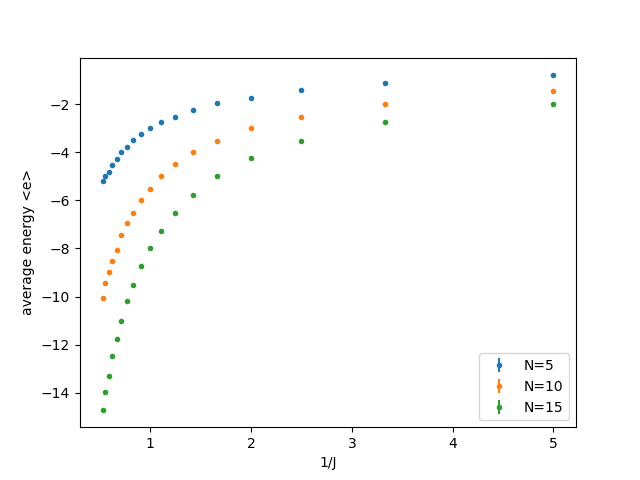
\includegraphics[width = .8\linewidth]{energy_vs_J^-1.png}
    \caption{average energy vs. $J^{-1}$}
    \label{fig:ener_J-1}
\end{figure}

You can see the simulated result in the plots \ref{fig:mag_J} and \ref{fig:ener_J} and the corresponding analytical result in the plots \ref{fig:anal_mag} and \ref{fig:anal_ener}. As can be seen, the simulated and analytical results are very similar. It is shown quite well how the curves of magnetization and energy approximate closer to the analytical results. 
Both analytical and simulated results show a phase transition at a certain point of J. From this point on, the mean magnetization starts to fall straight down from 1. For the average energy, the phase trasition can not be seen very well and it looks rather more like a linear behavior. If we plot it against $J^{-1}$ the plot shows more significant the trasition change of the energy.    

\end{enumerate}

\end{document}